\documentclass[10pt]{article} % For LaTeX2e
\usepackage{nips14submit_e,times}
\usepackage[letterpaper, margin = 1in]{geometry}
\usepackage{hyperref}
\usepackage{url}
\usepackage{graphicx}
\usepackage{float}


\title{Eyes Around The World - Learning to Alert and Cluster Live Webcams}


\newcommand{\fix}{\marginpar{FIX}}
\newcommand{\new}{\marginpar{NEW}}


\begin{document}
\maketitle

%\begin{abstract}
%Fill in abstract if there is space.
%\end{abstract}

\section{Introduction}
There are a large number of public live webcams that are accessible over the internet. A variety of content and objects from various places all around the world are being recorded by these webcams in real-time, but it is not feasible for a single person to browse through all of the webcams to search for content that is of interest. Our project aims to use Machine Learning algorithms to cluster and identify webcams of interest out of a large pool of webcams. This has relevance to security, surveillance and exploration applications where there is a need to filter through a large number of video streams to detect objects of interest. 

The input to our system is a stream of images from multiple webcams. For each webcam image, we use a Gaussian mixture model to model the background image, use to background model to extract foreground objects from the webcam image, and use a convolutional neural network to classify the detected objects. The output of our system is a display list of the top 5 webcams as ranked by the scoring algorithm for the webcams, which can be changed depending on the user input query. We also use K-means clustering to explore the different categories of webcams that exist in our dataset. 

\section{Related Work}
Several groups have previously looked at exploring and characterizing the network of webcams around the world. A previous effort was made to discover and characterize the locations and categories of webcams \cite{webcamnetwork} based on their geo-IP addresses and links from existing GIS databases. Our current work extends this effort to try to characterize webcams where there does not exist clean metadata and descriptions of the webcams. There has also been work in the area of image fusion \cite{billioneyes} of webcam images with data from Google StreetView and Google Earth images to provide additional context to existing images from a webcam. This was more aimed towards providing improved location-based services for mobile applications, whereas our work focuses on alerting webcams solely based off their data streams. 

The closest and most relevant previous work that has been conducted is real-time abnormality detection from multiple webcams \cite{huntingnessie}, where a nearest-neighbor model is used to create a image abnormality classifier based on simple image features. The distance/similarity metric used for nearest-neighbors clustering is based on outliers relative to a sample of past webcam images from varying time intervals, and is primarily based on image quadrants in a picture. Our work extends this by showing that it is possible to use object tracking methods by working on a pixel level instead of a quadrant level to detect objects, and our work differs in that our interest metric is primarily tied to the activity of a scene instead of abnormality relative to past images. 

Other related work is person identification from webcam images via semi-supervised learning \cite{personidentification}, where facial features are extracted from webcam images to locate track the position of people in those images. Our approach differs from this aspect in that we aim to track multiple kinds of objects instead. Work has also been done in using webcams to detect and monitor birds in the wild \cite{birddetection} using a median filter by defining the background as the median of the previous N frames. Our work uses a different method (model background as Gaussian mixture model) for object detection instead. 

\section{Dataset and Features}
Our data set consists of images logged from approximately 2000 publicly accessible, non-password-protected webcams, where query urls were scraped from the website opentopia.com \cite{opentopia}. Although we would ideally run our algorithms directly on live webcam streams, the bandwidth required to simultaneously process a meaningful number of webcams was prohibitively high. As a result, we logged images from those 2000 webcams at a 5 minute recording period over a duration of 1 month, and ran our algorithms on that dataset. 

The raw webcam images vary greatly in resolution - From as low to 240 x 180 to as high as 2048 x 1536. We log the webcam images in their native resolution for processing flexibility later on, and resize them to smaller resolutions (typically 300 x 300) as input into our system. Sample images from some webcams are shown below :

\begin{figure}[h]
\caption{Sample webcam images}
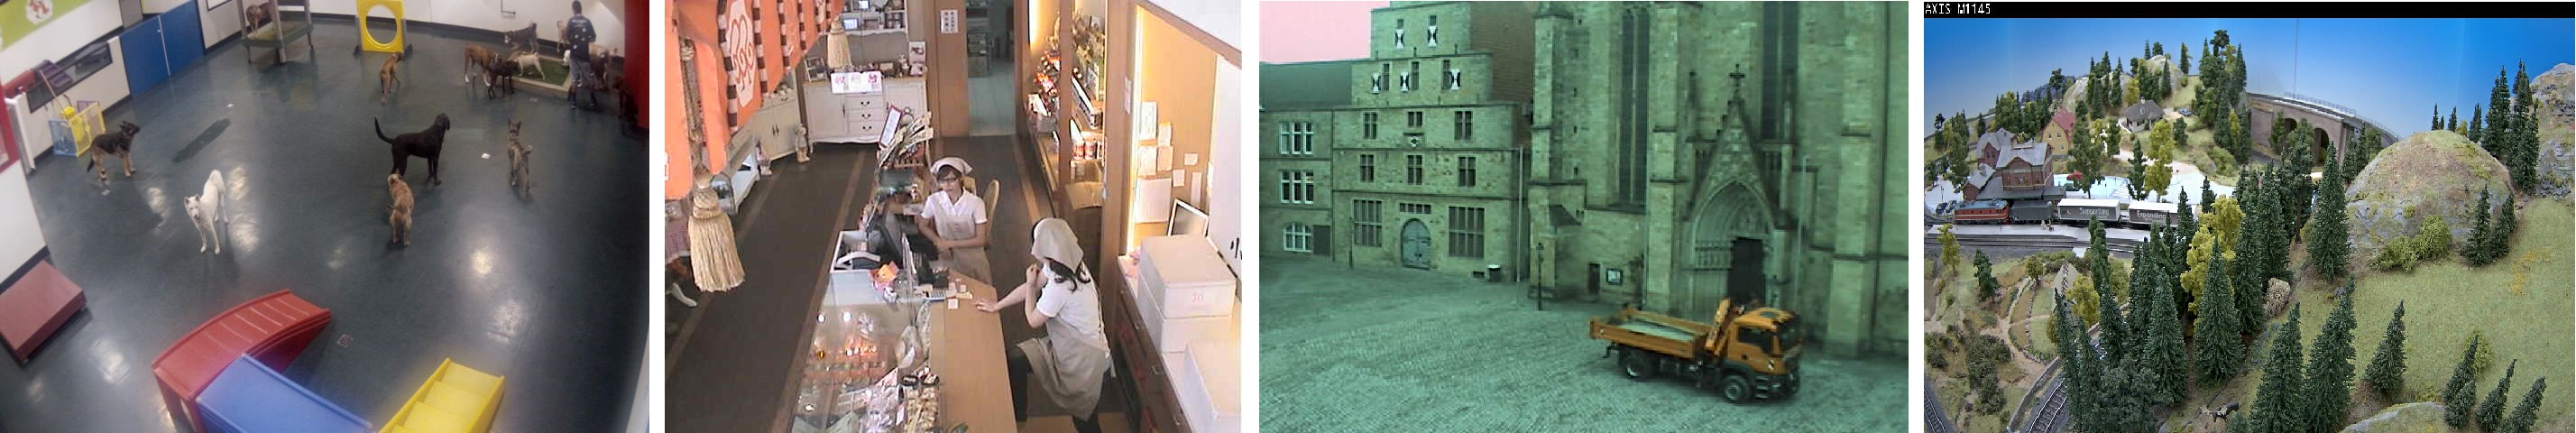
\includegraphics[scale = 0.25]{samples}
\end{figure}

\textcolor{red}{[SEAN to add some elaboration on features extracted for K-means clustering?]}

\section{Methods}
\subsection{Webcam ranking}
In order to rank webcams based on the activity of the objects recorded, it is necessary to separate foreground objects from the image background. To do this, we use OpenCV's BackgroundSubtractorMOG2() method to construct a background model for each pixel, and use it to classify pixels as foreground or background. The method implements the algorithm described in a paper by Zivkovic \cite{zivkovic} for background subtraction. The model is a generative model that uses a Gaussian mixture model (GMM) to model the background color distribution for each pixel. 

Let $\vec{x}^{(t)}$ be the value of a pixel at time $t$, and let $T$ be a time period over which samples are recorded. Define the training data set $\chi_T = \{\vec{x}^{(t)}, ... ,\vec{x}^{(t-T)}\} $. $\chi_T$ is updated with each new sample. An estimate of the background (BG) and foreground (FG) distribution can be modeled by a GMM with $M$ components :
\begin{equation}
\hat{p}(\vec{x}^{(t)} | \chi_T , BG+FG) = \sum_{m=1}^M \hat{\pi}_m \mathcal{N}(\vec{x} ; \hat{\vec{\mu}}_m ,  \hat{\sigma}_m^2 I)
\end{equation}
where $\hat{\vec{\mu}}_1 , .. , \hat{\vec{\mu}}_m$ are mean estimates and $\hat{\sigma}_1 , ... , \hat{\sigma}_m$ are variance estimates. $\hat{\pi}_m$ are the mixing weights that are non-negative and sum to 1. Given a new data sample $\vec{x}^{(t)}$, the parameters of the model can be updated recursively as \cite{zivkovic2}:
\begin{equation}
\hat{\pi}_m \leftarrow \hat{\pi}_m + \alpha ( o_m^{(t)} - \hat{\pi}_m) \\
\end{equation}
\begin{equation}
\hat{\vec{\mu}}_m \leftarrow \hat{\vec{\mu}}_m + o_m^{(t)} (\alpha / \hat{\pi}_m) \vec{\delta}_m \\
\end{equation}
\begin{equation}
\hat{\sigma}_m^2 \leftarrow + o_m^{(t)} (\alpha / \hat{\pi}_m)(  \vec{\delta}_m^T  \vec{\delta} - \hat{\sigma}_m^2)
\end{equation}
where $\vec{\delta} = \vec{x}^{(t)} - \hat{\vec{\mu}}_m$,  $\alpha$ is a exponential decay factor such that $\alpha \approx 1/T$ to limit influence of old data, and $o_m^{(t)}$ is defined as the "ownership". For a new sample, $o_m^{(t)}$ is set to 1 for the 'closest' component with largest $\hat{\pi}_m$ and others are set to zero, where 'closest' is based on the mahalanobis distance metric. The squared distance from the $m$-th component is calculated as $D_m^2 ( \vec{x}^{(t)}) = \vec{\delta}_m^T  \vec{\delta} / \hat{\sigma}_m^2$. 

Foreground objects usually correspond to some additional clusters with small weights $\hat{\pi}_m$. Thus, the background model can be approximated by the first $B$ largest clusters
\begin{equation}
p(\vec{x} | \chi_ , BG) \sim \sum_{m=1}^B \hat{\pi}_m \mathcal{N}(\vec{x} ; \hat{\vec{\mu}}_m ,  \hat{\sigma}_m^2 I)
\end{equation}

We use the background model to classify each pixel in the image as either being part of the foreground or background to obtain a foreground mask. We then fit contours around the sections of foreground object pixels using OpenCV's findContours() method. The contours are filtered based on size - Contours that are too small ($<$ 1\% of picture area) are attributed to noise, contours that are too large ($>$20\% of picture area) are attributed to pixel changes due illumination or webcam position, which are not of interest. \textcolor{red}{Example pics?}

A webcam's score is then calculated as the sum of contour areas as a percentage of the image size divided by the sum of contour arc lengths, Score = total contour area % / total contour length. We maximize for contour area to be able to show the largest / most number of objects after filtering. We minimize for contour length to reward convexity, as we found that large noisy artifacts in the webcam images tended to be highly non-convex in shape. \textcolor{red}{Example pics?}

\textcolor{red}{[SEAN to add methods for clustering + CNN]}

\section{Results / Discussion}
\subsection{Webcam ranking}
We present 2 sample snapshot results of the top 4/1000 webcams as ranked by our scoring algorithm. The webcam images with detected objects is shown on the top row, and the corresponding background image is shown in the bottom row. 
\begin{figure}[H]
\centering
\caption{Snapshot of top 4/1000 webcams from run 1 (left) and run 2 (right)}
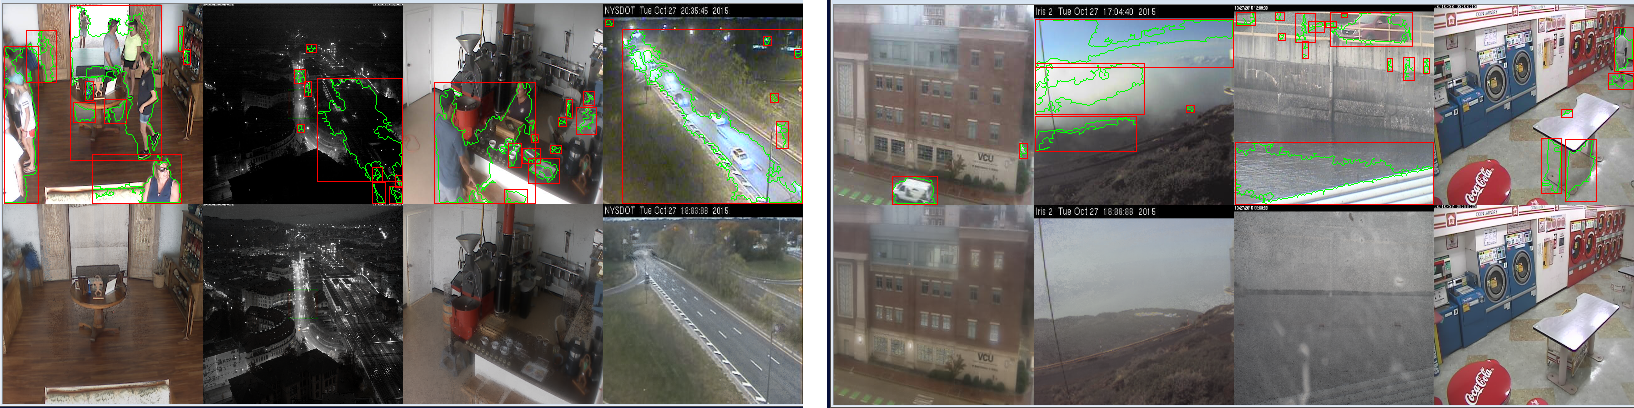
\includegraphics[scale = 0.5]{wc}
\end{figure}
We see that the algorithm returns qualitatively acceptable results - It is able to highlight clear changes and rise in activity of webcams, such as people filling into a room or traffic conditions changing. 

Even though we perform filtering on contours and on the scoring function to try to eliminate noise, there are still occurrences where our algorithm is influenced by image, lighting or webcam noise and ranks certain webcam images highly when there actually isn't any noticeable activity or changes. Several examples of webcam images that were ranked in the top 5/1000 are shown below :
\begin{figure}[H]
\centering
\caption{Examples of erroneously highly-ranked webcam images}
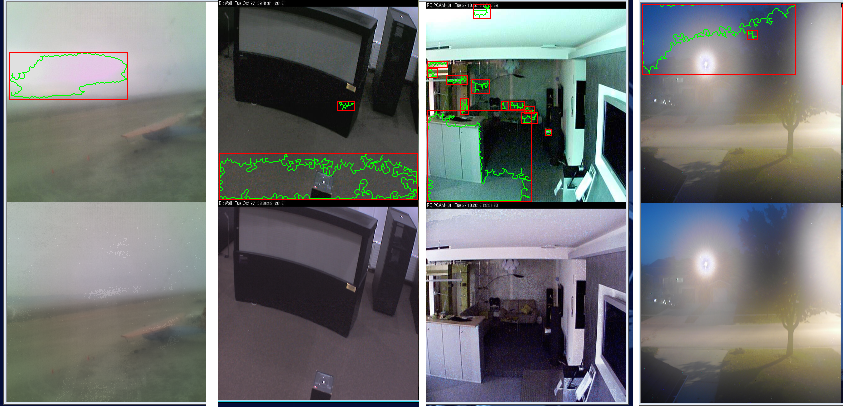
\includegraphics[scale = 0.5]{fails}
\end{figure}

\textcolor{red}{[SEAN to add results for clustering + CNN]}

\section{Conclusions / Future Work}
We have demonstrated a system to rank a large number of webcams using an interest metric that is based on the amount of activity that is currently recorded by a webcam. Webcam activity was quantified by the area of contours fit to foreground pixels classified by a Gaussian Mixture Model for the background model, and the interest metric was designed to reward the number, size and convexity of detected objects. 

One of the main bottlenecks to this project was the amount of GPU memory available to store webcam images. In order to be able to detect objects reliably, it is necessary to have the resolution of the images be above a certain size. However, the GPU memory required to process each image increases as the image resolution increases. At an image resolution of 300 x 300, we were able to simultaneously process a maximum of 1000 images at a time. Given extra computational resources, we would apply our system to the all 2000 webcams in the dataset.

\textcolor{red}{[SEAN to add future work for CNN]}


\begin{thebibliography}{9}
\bibitem{webcamnetwork}
Jacobs, Nathan, et al. "The global network of outdoor webcams: properties and applications." Proceedings of the 17th ACM SIGSPATIAL International Conference on Advances in Geographic Information Systems. ACM, 2009.

\bibitem{billioneyes}
Luo, Jiebo. "Vision with a billion eyes." Proceedings of the 2nd ACM international workshop on Geotagging and its applications in multimedia. ACM, 2013.

\bibitem{personidentification}
Balcan, Maria-Florina, et al. "Person identification in webcam images: An application of semi-supervised learning." (2005).

\bibitem{huntingnessie}
Breitenstein, Michael D., Helmut Grabner, and Luc Van Gool. "Hunting nessie-real-time abnormality detection from webcams." Computer Vision Workshops (ICCV Workshops), 2009 IEEE 12th International Conference on. IEEE, 2009.

\bibitem{birddetection}
Verstraeten, Willem W., et al. "Webcams for bird detection and monitoring: A demonstration study." Sensors 10.4 (2010): 3480-3503.

\bibitem{opentopia}
"Opentopia." Opentopia. Web. 10 Dec. 2015.

\bibitem{zivkovic}
Zivkovic, Zoran. "Improved adaptive Gaussian mixture model for background subtraction." Pattern Recognition, 2004. ICPR 2004. Proceedings of the 17th International Conference on. Vol. 2. IEEE, 2004.

\bibitem{zivkovic2}
Z.Zivkovic and F.van der Heijden, “Recursive Unsupervised Learning of Finite Mixture Models”, IEEE Trans. on PAMI, vol.26., no.5, 2004.

\end{thebibliography}

\end{document}
